\documentclass[11pt,a4paper]{report}
\usepackage[textwidth=37em,vmargin=30mm]{geometry}
\usepackage{calc,xunicode,amsmath,amssymb,paralist,enumitem,tabu,booktabs,datetime2,xeCJK,xeCJKfntef,listings}
\usepackage{tocloft,fancyhdr,tcolorbox,xcolor,graphicx,eso-pic,xltxtra,xelatexemoji}

\newcommand{\envyear}[0]{2025}
\newcommand{\envdatestr}[0]{2025-09-24}
\newcommand{\envfinaldir}[0]{webdb/2025/20250924/final}

\usepackage[hidelinks]{hyperref}
\hypersetup{
    colorlinks=false,
    pdfpagemode=FullScreen,
    pdftitle={Web Digest - \envdatestr}
}

\setlength{\cftbeforechapskip}{10pt}
\renewcommand{\cftchapfont}{\rmfamily\bfseries\large\raggedright}
\setlength{\cftbeforesecskip}{2pt}
\renewcommand{\cftsecfont}{\sffamily\small\raggedright}

\setdefaultleftmargin{2em}{2em}{1em}{1em}{1em}{1em}

\usepackage{xeCJK,xeCJKfntef}
\xeCJKsetup{PunctStyle=plain,RubberPunctSkip=false,CJKglue=\strut\hskip 0pt plus 0.1em minus 0.05em,CJKecglue=\strut\hskip 0.22em plus 0.2em}
\XeTeXlinebreaklocale "zh"
\XeTeXlinebreakskip = 0pt


\setmainfont{Brygada 1918}
\setromanfont{Brygada 1918}
\setsansfont{IBM Plex Sans}
\setmonofont{JetBrains Mono NL}
\setCJKmainfont{Noto Serif CJK SC}
\setCJKromanfont{Noto Serif CJK SC}
\setCJKsansfont{Noto Sans CJK SC}
\setCJKmonofont{Noto Sans CJK SC}

\setlength{\parindent}{0pt}
\setlength{\parskip}{8pt}
\linespread{1.15}

\lstset{
	basicstyle=\ttfamily\footnotesize,
	numbersep=5pt,
	backgroundcolor=\color{black!5},
	showspaces=false,
	showstringspaces=false,
	showtabs=false,
	tabsize=2,
	captionpos=b,
	breaklines=true,
	breakatwhitespace=true,
	breakautoindent=true,
	linewidth=\textwidth
}






\newcommand{\coverpic}[2]{
    % argv: itemurl, authorname
    Cover photo by #2~~(\href{#1}{#1})
}
\newcommand{\makeheader}[0]{
    \begin{titlepage}
        % \newgeometry{hmargin=15mm,tmargin=21mm,bmargin=12mm}
        \begin{center}
            
            \rmfamily\scshape
            \fontspec{BaskervilleF}
            \fontspec{Old Standard}
            \fontsize{59pt}{70pt}\selectfont
            WEB\hfill DIGEST
            
            \vfill
            % \vskip 30pt
            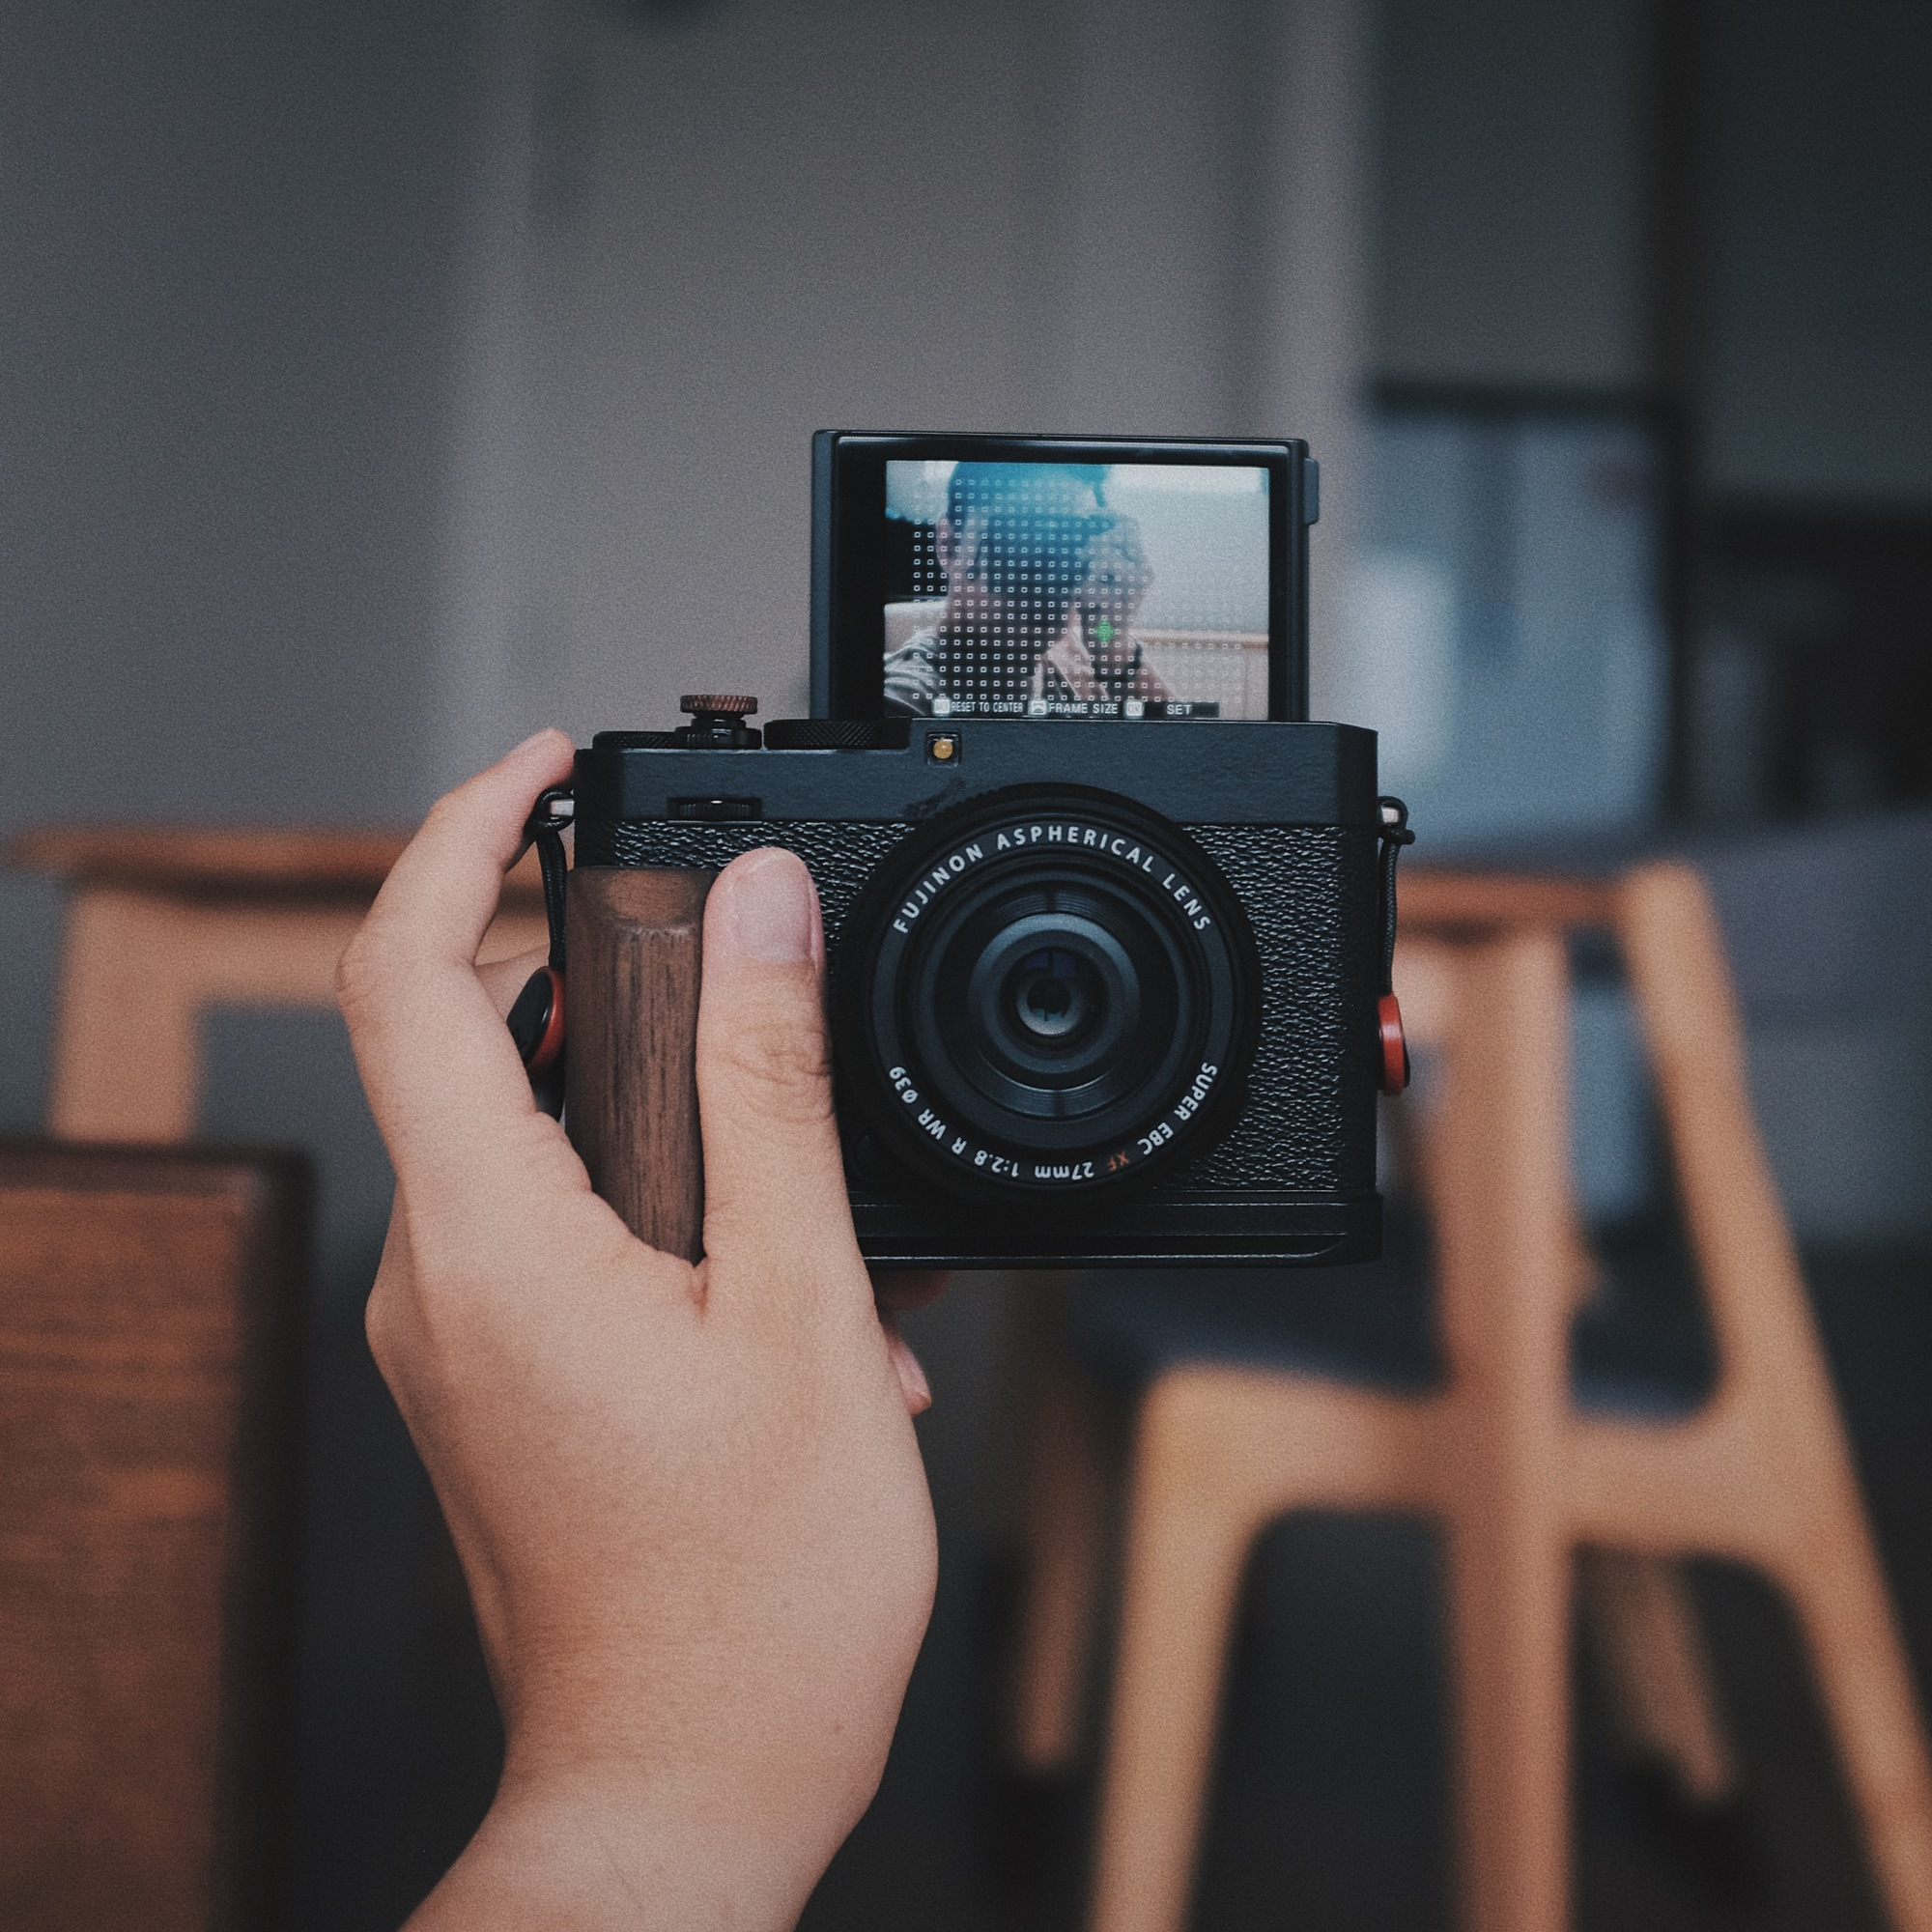
\includegraphics[width=\linewidth]{\envfinaldir/coverpic-prod.jpg}\par
            % \vskip 30pt
            \vfill

            \normalsize\rmfamily\scshape
            \copyright{} The Web Digest Project \hfill\large \envdatestr
        \end{center}
    \end{titlepage}
    % \restoregeometry
}
\newcommand{\simplehref}[1]{%
    \textcolor{blue!80!green}{\href{#1}{#1}}%
}
\renewcommand{\contentsname}{\center\Huge\sffamily\bfseries Contents\par\vskip 20pt}
\newcounter{ipartcounter}
\setcounter{ipartcounter}{0}
\newcommand{\ipart}[1]{
    % \vskip 20pt
    \clearpage
    \stepcounter{ipartcounter}
    \phantomsection
    \addcontentsline{toc}{chapter}{#1}
    % \begin{center}
    %     \Huge
    %     \sffamily\bfseries
    %     #1
    % \end{center}
    % \vskip 20pt plus 7pt
}
\newcounter{ichaptercounter}
\setcounter{ichaptercounter}{0}
\newcommand{\ichapter}[1]{
    % \vskip 20pt
    \clearpage
    \stepcounter{ichaptercounter}
    \phantomsection
    \addcontentsline{toc}{section}{\numberline{\arabic{ichaptercounter}}#1}
    \begin{center}
        \Huge
        \sffamily\bfseries
        #1
    \end{center}
    \vskip 20pt plus 7pt
}
\newcommand{\entrytitlefont}[1]{\subsection*{\raggedright\Large\sffamily\bfseries#1}}
\newcommand{\entryitemGeneric}[2]{
    % argv: title, url
    \parbox{\linewidth}{
        \entrytitlefont{#1}\par\vskip 5pt
        \footnotesize\ttfamily\mdseries
        \simplehref{#2}
    }\vskip 11pt plus 11pt minus 1pt
}
\newcommand{\entryitemGithub}[3]{
    % argv: title, url, desc
    \parbox{\linewidth}{
        \entrytitlefont{#1}\par\vskip 5pt
        \footnotesize\ttfamily\mdseries
        \simplehref{#2}\par\vskip 5pt
        \small\rmfamily\mdseries#3
    }\vskip 11pt plus 11pt minus 1pt
}
\newcommand{\entryitemAp}[3]{
    % argv: title, url, desc
    \parbox{\linewidth}{
        \entrytitlefont{#1}\par\vskip 5pt
        \footnotesize\ttfamily\mdseries
        \simplehref{#2}\par\vskip 5pt
        \small\rmfamily\mdseries#3
    }\vskip 11pt plus 11pt minus 1pt
}
\newcommand{\entryitemHackernews}[3]{
    % argv: title, hnurl, rawurl
    % \parbox{\linewidth}{
    %     \entrytitlefont{#1}\par\vskip 5pt
    %     \footnotesize\ttfamily\mdseries
    %     \simplehref{#3}\par
    %     \textcolor{black!50}{\href{#2}{#2}}
    % }\vskip 11pt plus 11pt minus 1pt
    \begin{minipage}{\linewidth}
            \entrytitlefont{#1}\par\vskip 5pt
            \footnotesize\ttfamily\mdseries
            \simplehref{#3}\par
            \textcolor{black!50}{\href{#2}{#2}}
    \end{minipage}\par\vskip 11pt plus 11pt minus 1pt
}







\begin{document}

\makeheader

\tableofcontents\clearpage




\ipart{Developers}
\ichapter{Hacker News}
\entryitemTwoLinks{Qwen3-VL}{https://news.ycombinator.com/item?id=45352672}{https://qwen.ai/blog?id=99f0335c4ad9ff6153e517418d48535ab6d8afef\&from=research.latest-advancements-list}

\entryitemTwoLinks{I'm leaving Ruby Central}{https://news.ycombinator.com/item?id=45352432}{https://gist.github.com/simi/349d881d16d3d86947945615a47c60ca}

\entryitemTwoLinks{YouTube says it'll bring back creators banned for Covid and election content}{https://news.ycombinator.com/item?id=45352213}{https://www.businessinsider.com/youtube-reinstate-channels-banned-over-covid-content-policies-2025-9}

\entryitemTwoLinks{consumed.today}{https://news.ycombinator.com/item?id=45351446}{https://consumed.today/}

\entryitemTwoLinks{Denmark wants to push through Chat Control}{https://news.ycombinator.com/item?id=45351405}{https://netzpolitik.org/2025/internes-protokoll-daenemark-will-chatkontrolle-durchdruecken/}

\entryitemTwoLinks{Find SF parking cops}{https://news.ycombinator.com/item?id=45350690}{https://walzr.com/sf-parking/}

\entryitemTwoLinks{Android users can now use conversational editing in Google Photos}{https://news.ycombinator.com/item?id=45349848}{https://blog.google/products/photos/android-conversational-editing-google-photos/}

\entryitemTwoLinks{If you are reading this obituary, it looks like I'm dead}{https://news.ycombinator.com/item?id=45348700}{https://framinghamsource.com/index.php/2025/09/22/linda-m-brossi-murphy/}

\entryitemTwoLinks{Always Invite Anna}{https://news.ycombinator.com/item?id=45348495}{https://sharif.io/anna-alexei}

\entryitemTwoLinks{Shopify, pulling strings at Ruby Central, forces Bundler and RubyGems takeover}{https://news.ycombinator.com/item?id=45348390}{https://joel.drapper.me/p/rubygems-takeover/}

\entryitemTwoLinks{From MCP to shell: MCP auth flaws enable RCE in Claude Code, Gemini CLI and more}{https://news.ycombinator.com/item?id=45348183}{https://verialabs.com/blog/from-mcp-to-shell/}

\entryitemTwoLinks{Launch HN: Strata (YC X25) – One MCP server for AI to handle thousands of tools}{https://news.ycombinator.com/item?id=45347914}{https://news.ycombinator.com/item?id=45347914}

\entryitemTwoLinks{Getting AI to work in complex codebases}{https://news.ycombinator.com/item?id=45347532}{https://github.com/humanlayer/advanced-context-engineering-for-coding-agents/blob/main/ace-fca.md}

\entryitemTwoLinks{x402 — An open protocol for internet-native payments}{https://news.ycombinator.com/item?id=45347335}{https://www.x402.org/}

\entryitemTwoLinks{Libghostty is coming}{https://news.ycombinator.com/item?id=45347117}{https://mitchellh.com/writing/libghostty-is-coming}

\entryitemTwoLinks{Restrictions on house sharing by unrelated roommates}{https://news.ycombinator.com/item?id=45347043}{https://marginalrevolution.com/marginalrevolution/2025/08/the-war-on-roommates-why-is-sharing-a-house-illegal.html}

\entryitemTwoLinks{MrBeast Failed to Disclose Ads and Improperly Collected Children's Data}{https://news.ycombinator.com/item?id=45346950}{https://bbbprograms.org/media/newsroom/decisions/mrbeast-feastables}

\entryitemTwoLinks{Zig feels more practical than Rust for real-world CLI tools}{https://news.ycombinator.com/item?id=45346387}{https://dayvster.com/blog/why-zig-feels-more-practical-than-rust-for-real-world-cli-tools/}

\entryitemTwoLinks{Getting More Strategic}{https://news.ycombinator.com/item?id=45346219}{https://cate.blog/2025/09/23/getting-more-strategic/}

\entryitemTwoLinks{Mesh: I tried Htmx, then ditched it}{https://news.ycombinator.com/item?id=45345950}{https://ajmoon.com/posts/mesh-i-tried-htmx-then-ditched-it}\ichapter{Phoronix}
\entryitemGeneric{\hskip 0pt{}Haptic Touchpad Support Expected For Linux 6.18}{https://www.phoronix.com/news/Haptic-Touchpad-Linux-6.18}

\entryitemGeneric{\hskip 0pt{}Bytedance Proposes "Parker" For Linux: Multiple Kernels Running Simultaneously}{https://www.phoronix.com/news/Linux-Parker-Proposal}

\entryitemGeneric{\hskip 0pt{}Running The Bcachefs DKMS Modules On Ubuntu Linux}{https://www.phoronix.com/review/bcachefs-617-dkms}

\entryitemGeneric{\hskip 0pt{}Linux 6.18 To Improve Support For Apple's A11, Other Apple Silicon Improvements}{https://www.phoronix.com/news/Apple-Silicon-Linux-6.18-Ready}

\entryitemGeneric{\hskip 0pt{}AMD Versal NET DDR EDAC Driver Ready For Linux 6.18}{https://www.phoronix.com/news/AMD-Versal-NET-EDAC-Linux-6.18}

\entryitemGeneric{\hskip 0pt{}New Patches Optimize EXT4 Online Defragmentation For Better Performance}{https://www.phoronix.com/news/EXT4-Faster-Online-Defrag}

\entryitemGeneric{\hskip 0pt{}Mesa 25.3 Lands SPIR-V Shader Replacement Support}{https://www.phoronix.com/news/Mesa-SPIR-V-Shader-Replacement}

\entryitemGeneric{\hskip 0pt{}FFmpeg Lands Support For AHX, ADPCM Silicon Graphics N64 Decoder}{https://www.phoronix.com/news/FFmpeg-AHX-Support}

\entryitemGeneric{\hskip 0pt{}Qt 6.10 RC Available For Testing With Native PipeWire Audio Back-End}{https://www.phoronix.com/news/Qt-6.10-RC}


\ipart{Developers~~~~(zh-Hans)}
\ichapter{Solidot}
\entryitemGeneric{\hskip 0pt{}多地推进采集男性居民血样}{https://www.solidot.org/story?sid=82395}

\entryitemGeneric{\hskip 0pt{}BMI 指数过低死亡风险可能更高}{https://www.solidot.org/story?sid=82394}

\entryitemGeneric{\hskip 0pt{}TikTok 算法将在美国重新训练}{https://www.solidot.org/story?sid=82393}

\entryitemGeneric{\hskip 0pt{}Google TV 加入 Gemini AI 助手}{https://www.solidot.org/story?sid=82392}

\entryitemGeneric{\hskip 0pt{}Windows 11 支持将视频设为墙纸}{https://www.solidot.org/story?sid=82390}

\entryitemGeneric{\hskip 0pt{}英伟达向 OpenAI 投资千亿美元}{https://www.solidot.org/story?sid=82389}

\entryitemGeneric{\hskip 0pt{}埃及总统赦免 Alaa Abdel Fattah}{https://www.solidot.org/story?sid=82388}

\entryitemGeneric{\hskip 0pt{}Multi-Kernel 架构支持代码公开}{https://www.solidot.org/story?sid=82386}

\entryitemGeneric{\hskip 0pt{}Tails 7.0 释出}{https://www.solidot.org/story?sid=82385}

\entryitemGeneric{\hskip 0pt{}BlockBlasters 游戏补丁被发现含有恶意程序}{https://www.solidot.org/story?sid=82384}

\entryitemGeneric{\hskip 0pt{}中国海军成功测试舰载机电磁弹射}{https://www.solidot.org/story?sid=82383}

\entryitemGeneric{\hskip 0pt{}英国银行仍然运行 1960 年代写的代码}{https://www.solidot.org/story?sid=82382}

\entryitemGeneric{\hskip 0pt{}西雅图艰难应对科技工作减少}{https://www.solidot.org/story?sid=82381}

\entryitemGeneric{\hskip 0pt{}天文学家在地球附近发现一颗准卫星}{https://www.solidot.org/story?sid=82380}

\entryitemGeneric{\hskip 0pt{}微软的 Entra ID 漏洞可能造成灾难性的后果}{https://www.solidot.org/story?sid=82379}

\entryitemGeneric{\hskip 0pt{}微软向用户推送 Gaming Copilot,中国地区除外 }{https://www.solidot.org/story?sid=82378}

\entryitemGeneric{\hskip 0pt{}退休有助于改善心理健康,但并非人人如此}{https://www.solidot.org/story?sid=82377}

\entryitemGeneric{\hskip 0pt{}教宗拒绝授权创建一个 AI 教宗}{https://www.solidot.org/story?sid=82376}

\entryitemGeneric{\hskip 0pt{}地中海饮食与更低的牙龈疾病风险相关}{https://www.solidot.org/story?sid=82375}

\entryitemGeneric{\hskip 0pt{}OpenAI 研究人员称 AI 幻觉在数学上是不可避免的}{https://www.solidot.org/story?sid=82374}\ichapter{V2EX}
\entryitemGeneric{\hskip 0pt{}[推广] 可灵 2.5 昨天晚上刚上线,听说能硬刚 veo3 和 runway?}{https://www.v2ex.com/t/1161405}

\entryitemGeneric{\hskip 0pt{}[macOS] 26 已经装了几天了,明显觉得日常占用 cpu 变高,续航也变短,流畅度也降低了。}{https://www.v2ex.com/t/1161403}

\entryitemGeneric{\hskip 0pt{}[程序员] 升级 Gnome 49,发现自带的免费软件的也是很不错的}{https://www.v2ex.com/t/1161402}

\entryitemGeneric{\hskip 0pt{}[问与答] uBar – 替换 Dock 为 Windows 开始菜单样式[OS X]}{https://www.v2ex.com/t/1161401}

\entryitemGeneric{\hskip 0pt{}[问与答] win11 无限重启求助}{https://www.v2ex.com/t/1161400}

\entryitemGeneric{\hskip 0pt{}[Apple] 几年了,还是不能适应 iPad 音量键跟随旋转方向改变}{https://www.v2ex.com/t/1161399}

\entryitemGeneric{\hskip 0pt{}[求职] 25 年秋季职业交易员招募:魔界之门}{https://www.v2ex.com/t/1161398}

\entryitemGeneric{\hskip 0pt{}[生活] 深夜碎碎念——人生真是如梦啊}{https://www.v2ex.com/t/1161397}

\entryitemGeneric{\hskip 0pt{}[招商银行] 招行 app 换上 iOS26 动效了 [非掌上生活]}{https://www.v2ex.com/t/1161396}

\entryitemGeneric{\hskip 0pt{}[程序员] 预算要多少? odoo 客户端 需要支持 全部官方客户端(apk, ipa)支持功能 或大部分功能?请报价}{https://www.v2ex.com/t/1161395}

\entryitemGeneric{\hskip 0pt{}[微信] [深夜不吐不快] 微信小程序是怎么变成一座屎山的?他们未来有没有可能重构?}{https://www.v2ex.com/t/1161394}

\entryitemGeneric{\hskip 0pt{}[分享发现] 炒了美股之后是不是都觉得巴菲特也就那样?}{https://www.v2ex.com/t/1161392}

\entryitemGeneric{\hskip 0pt{}[酷工作] 交个朋友,为两个孵化器项目找技术负责人}{https://www.v2ex.com/t/1161391}

\entryitemGeneric{\hskip 0pt{}[Apple] 用了几年的巨魔微信多开,今天被检测了}{https://www.v2ex.com/t/1161389}

\entryitemGeneric{\hskip 0pt{}[问与答] 喜欢一个女生的第一感觉是什么?}{https://www.v2ex.com/t/1161387}

\entryitemGeneric{\hskip 0pt{}[宽带症候群] 成都电信限 UDP 上传}{https://www.v2ex.com/t/1161386}

\entryitemGeneric{\hskip 0pt{}[奇思妙想] 折腾了这么多笔记软件,最终还是回到了果子自带的备忘录}{https://www.v2ex.com/t/1161385}

\entryitemGeneric{\hskip 0pt{}[酷工作] 数据管道开发工程师(Golang/ Python ),上海虹口区, GenAI 公司(一年内四轮融资,市值一亿美金+)}{https://www.v2ex.com/t/1161384}

\entryitemGeneric{\hskip 0pt{}[推广] Claude code 平价中转站,限时限量放送}{https://www.v2ex.com/t/1161382}

\entryitemGeneric{\hskip 0pt{}[Apple] 继 macOS 26 后, iOS 26 也在国内成功连上 6GHz Wi-Fi 了}{https://www.v2ex.com/t/1161381}

\entryitemGeneric{\hskip 0pt{}[问与答] 想买个小主机,跑全闪 nas 和一些 docker,有推荐的主机么?}{https://www.v2ex.com/t/1161379}

\entryitemGeneric{\hskip 0pt{}[NAS] 我的 NAS omv5.6.13 系统盘坏掉了,怎么恢复 raid 盘中的数据?}{https://www.v2ex.com/t/1161378}

\entryitemGeneric{\hskip 0pt{}[问与答] 感觉我的手机信号特别差}{https://www.v2ex.com/t/1161377}

\entryitemGeneric{\hskip 0pt{}[VPS] 想自己开个 claude code relay 服务,求 vps 推荐}{https://www.v2ex.com/t/1161376}

\entryitemGeneric{\hskip 0pt{}[宽带症候群] 有哪些大厂官方手机端 APP 有 PCDN 行为?}{https://www.v2ex.com/t/1161375}

\entryitemGeneric{\hskip 0pt{}[问与答] 闲鱼中的低价 icloud 是什么原理?}{https://www.v2ex.com/t/1161373}

\entryitemGeneric{\hskip 0pt{}[招商银行] 都 2025 年了,怎么招商银行一网通支付页面还在使用陈旧的 ActiveX 浏览器插件技术呢?}{https://www.v2ex.com/t/1161372}

\entryitemGeneric{\hskip 0pt{}[生活] 个体工商户的经营所得税减半征收也比工资税高?}{https://www.v2ex.com/t/1161369}

\entryitemGeneric{\hskip 0pt{}[宽带症候群] 国内 IPv4 中转机 VS. 购买流量卡}{https://www.v2ex.com/t/1161368}

\entryitemGeneric{\hskip 0pt{}[酷工作] 资深 Android 开发 [深圳/可远程]}{https://www.v2ex.com/t/1161367}

\entryitemGeneric{\hskip 0pt{}[程序员] 发现 autohotkey 这东西把 Go 写的命令行包装成 GUI 真是神器}{https://www.v2ex.com/t/1161366}

\entryitemGeneric{\hskip 0pt{}[Windows] Windows 有没有像 Mac mouse fix 或者 Better mouse 这样的鼠标侧键自定义软件?}{https://www.v2ex.com/t/1161364}

\entryitemGeneric{\hskip 0pt{}[酷工作] [苏州昆山] 招聘 Golang 高级开发工程师(物联网平台方向)}{https://www.v2ex.com/t/1161363}

\entryitemGeneric{\hskip 0pt{}[Apple] macos26 史诗级更新,我愿称之为最强的功能}{https://www.v2ex.com/t/1161362}

\entryitemGeneric{\hskip 0pt{}[随想] AGI 时代,人类劳动价值不再由劳动时间与稀缺衡量.........}{https://www.v2ex.com/t/1161361}

\entryitemGeneric{\hskip 0pt{}[iPhone] 如何快速把旧 iPhone 转移到新 iPhone}{https://www.v2ex.com/t/1161360}

\entryitemGeneric{\hskip 0pt{}[职场话题] Web3 对于 iOS 开发 到底是怎样一个方向?}{https://www.v2ex.com/t/1161359}

\entryitemGeneric{\hskip 0pt{}[加密货币] 有部分 U 在钱包里因缺乏 Gas 费而进退两难,何解?}{https://www.v2ex.com/t/1161358}

\entryitemGeneric{\hskip 0pt{}[酷工作] [招聘] React Native 工程师(广告归因 \& 平台集成方向)prefer 全职,可远程!}{https://www.v2ex.com/t/1161357}

\entryitemGeneric{\hskip 0pt{}[问与答] 大家现在线下支付是用微信还是支付宝多呀?}{https://www.v2ex.com/t/1161356}

\entryitemGeneric{\hskip 0pt{}[分享发现] 小白的香港开户总结,附旅游攻略}{https://www.v2ex.com/t/1161355}

\entryitemGeneric{\hskip 0pt{}[Apple] 有没有人知道这个屏幕时间是怎么计算的?}{https://www.v2ex.com/t/1161354}

\entryitemGeneric{\hskip 0pt{}[程序员] PaaS IaaS SaaS FaaS 大佬们,这些怎么念才显得不是新手}{https://www.v2ex.com/t/1161352}

\entryitemGeneric{\hskip 0pt{}[支付宝] 支付宝广告都这么写了嘛,直接写股票开户申请申请被驳回}{https://www.v2ex.com/t/1161351}

\entryitemGeneric{\hskip 0pt{}[问与答] 今年的车险为啥上涨这么多?}{https://www.v2ex.com/t/1161350}

\entryitemGeneric{\hskip 0pt{}[Apple] 如何解决 iOS macOS 26 检查更新一直在转圈?}{https://www.v2ex.com/t/1161349}

\entryitemGeneric{\hskip 0pt{}[全球工单系统] alibabacloud 炸了?}{https://www.v2ex.com/t/1161347}

\entryitemGeneric{\hskip 0pt{}[问与答] pixel 1 传大视频到 google photo 的问题}{https://www.v2ex.com/t/1161346}

\entryitemGeneric{\hskip 0pt{}[分享发现] 把自己变成安卓人吧😄}{https://www.v2ex.com/t/1161344}

\entryitemGeneric{\hskip 0pt{}[问与答] 希望发明腾讯信用分的产品经理被台风桦加沙吹走,芜湖}{https://www.v2ex.com/t/1161343}


\ipart{Generic News}







\clearpage
\leavevmode\vfill
\footnotesize

Copyright \copyright{} 2023-2025 Neruthes and other contributors.

This document is published with CC BY-NC-ND 4.0 license.

The entries listed in this newsletter may be copyrighted by their respective creators.

This newsletter is generated by the Web Digest project.

The newsletters are also delivered via Telegram channel \CJKunderline{\href{https://t.me/webdigestchannel}{https://t.me/webdigestchannel}}.\\
RSS feed is available at \CJKunderline{\href{https://webdigest.pages.dev/rss.xml}{https://webdigest.pages.dev/rss.xml}}.

This newsletter is available in PDF at
\CJKunderline{\href{https://webdigest.pages.dev/}{https://webdigest.pages.dev/}}.

The source code being used to generate this newsletter is available at\\
\CJKunderline{\href{https://github.com/neruthes/webdigest}{https://github.com/neruthes/webdigest}}.

This newsletter is also available in
\CJKunderline{\href{http://webdigest.pages.dev/readhtml/\envyear/WebDigest-20250924.html}{HTML}} and
\CJKunderline{\href{https://github.com/neruthes/webdigest/blob/master/markdown/\envyear/WebDigest-20250924.md}{Markdown}}.


\coverpic{https://unsplash.com/photos/a-room-with-a-table-and-a-mirror-x4G\_Kdo6sY4}{Neon Wang}


\end{document}
